% answers.tex —— 2013 年·上海卷·文科 · 参考答案与详细解析片段
% 由 tools/generate_projects.py 依来源总账自 2013/2013_数学真题_上海文_试题.md + 2013/2013_数学真题_上海文_解析正文.md + 2013/2013_数学真题_上海文_答案要点.md 生成，勿手改（改源 MD 后重跑）


\begin{answer}
\gksolhead{1}{}

\textbf{题目}：

不等式 $\dfrac{x}{2x-1}<0$ 的解为\gkblank{}。

\Needspace{4\baselineskip}
\textbf{解析}
\Needspace{5\baselineskip}
分母 $2x-1\neq0$。在 $2x-1$ 的符号确定的前提下，原不等式等价于
\nopagebreak[4]
\[x(2x-1)<0.\]
\Needspace{5\baselineskip}
二次方程 $x(2x-1)=0$ 的两根为 $0$ 与 $\dfrac12$，且二次项系数为正，故解集为
\nopagebreak[4]
\[0<x<\frac12,\]
即 $\left(0,\dfrac12\right)$。也可直接列表：$x<0$ 时分子负、分母负，商为正；$0<x<\dfrac12$ 时分子正、分母负，商为负；$x>\dfrac12$ 时商为正。

\gkanswer{答案：$\left(0,\dfrac12\right)$。由 $\dfrac{x}{2x-1}<0$ 得 $x(2x-1)<0$，两根为 $0$ 与 $\dfrac12$，故 $0<x<\dfrac12$。}

\end{answer}
\begin{answer}
\gksolhead{2}{}

\textbf{题目}：

在等差数列 $\{a_n\}$ 中，若 $a_1+a_2+a_3+a_4=30$，则 $a_2+a_3=$\gkblank{}。

\Needspace{4\baselineskip}
\textbf{解析}
\Needspace{5\baselineskip}
等差数列中下标和相等的两项和相等：
\nopagebreak[4]
\[a_1+a_4=a_2+a_3.\]
\Needspace{5\baselineskip}
由 $a_1+a_2+a_3+a_4=30$ 得
\nopagebreak[4]
\[2(a_2+a_3)=30,\]
故 $a_2+a_3=15$。数值复核：取 $a_1=3$，$d=6$，则 $3+9+15+21=48\neq30$；取 $a_1=0$，$d=5$，则 $0+5+10+15=30$，此时 $a_2+a_3=15$。

\gkanswer{答案：$15$。由 $a_1+a_4=a_2+a_3$ 得 $2(a_2+a_3)=30$，故 $a_2+a_3=15$。}

\end{answer}
\begin{answer}
\gksolhead{3}{}

\textbf{题目}：

设 $m\in\mathbf R$，$m^2+m-2+(m^2-1)\mathrm i$ 是纯虚数，其中 $\mathrm i$ 是虚数单位，则 $m=$\gkblank{}。

\Needspace{4\baselineskip}
\textbf{解析}
\Needspace{5\baselineskip}
设 $z=m^2+m-2+(m^2-1)\mathrm i$。$z$ 为纯虚数，当且仅当
\nopagebreak[4]
\[\begin{cases}
m^2+m-2=0,\\
m^2-1\neq0.
\end{cases}\]
第一式因式分解得 $(m-1)(m+2)=0$，即 $m=1$ 或 $m=-2$；第二式给出 $m\neq\pm1$。因此 $m=-2$。

\gkanswer{答案：$-2$。纯虚数要求实部为 $0$ 且虚部不为 $0$：$m^2+m-2=0$ 给出 $m=1$ 或 $m=-2$；$m^2-1\neq0$ 排除 $m=\pm1$，故 $m=-2$。}

\end{answer}
\begin{answer}
\gksolhead{4}{}

\textbf{题目}：

若 $\begin{vmatrix}x&2\\1&1\end{vmatrix}=0$，$\begin{vmatrix}x&y\\1&1\end{vmatrix}=1$，则 $x+y=$\gkblank{}。

\Needspace{4\baselineskip}
\textbf{解析}
\Needspace{5\baselineskip}
二阶行列式按定义展开：
\nopagebreak[4]
\[\begin{vmatrix}x&2\\1&1\end{vmatrix}=x\cdot1-2\cdot1=x-2,\]
\Needspace{5\baselineskip}
由 $x-2=0$ 得 $x=2$。又
\nopagebreak[4]
\[\begin{vmatrix}x&y\\1&1\end{vmatrix}=x-y,\]
由 $x-y=1$ 得 $y=x-1=1$。故 $x+y=3$。

\gkanswer{答案：$3$。由 $x-2=0$ 得 $x=2$；由 $x-y=1$ 得 $y=1$，故 $x+y=3$。}

\end{answer}
\begin{answer}
\gksolhead{5}{}

\textbf{题目}：

已知 $\triangle ABC$ 的内角 $A$、$B$、$C$ 所对的边分别是 $a$、$b$、$c$。若 $a^2+ab+b^2-c^2=0$，则角 $C$ 的大小是\gkblank{}。

\Needspace{4\baselineskip}
\textbf{解析}
\Needspace{5\baselineskip}
由 $a^2+ab+b^2-c^2=0$ 得
\nopagebreak[4]
\[c^2=a^2+b^2+ab.\]
\Needspace{5\baselineskip}
而余弦定理给出 $c^2=a^2+b^2-2ab\cos C$，两式比较得
\nopagebreak[4]
\[-2ab\cos C=ab,\]
\Needspace{5\baselineskip}
因 $a,b>0$ 可约去 $ab$，得 $\cos C=-\dfrac12$。又 $C\in(0,\pi)$，故
\nopagebreak[4]
\[C=\frac{2\pi}3.\]

\gkanswer{答案：$\dfrac{2\pi}3$。由 $c^2=a^2+b^2+ab$ 与余弦定理 $c^2=a^2+b^2-2ab\cos C$ 得 $\cos C=-\dfrac12$，故 $C=\dfrac{2\pi}3$。}

\end{answer}
\begin{answer}
\gksolhead{6}{}

\textbf{题目}：

某学校高一年级男生人数占该年级学生人数的 $40\%$。在一次考试中，男、女生平均分数分别为 $75$、$80$，则这次考试该年级学生平均分数为\gkblank{}。

\Needspace{4\baselineskip}
\textbf{解析}
\Needspace{5\baselineskip}
设该年级学生总数为 $N$，则男生 $0.4N$ 人，女生 $0.6N$ 人。总分为
\nopagebreak[4]
\[0.4N\cdot75+0.6N\cdot80=N(30+48)=78N,\]
故平均分为 $78$。

\gkanswer{答案：$78$。按人数加权：$0.4\times75+0.6\times80=30+48=78$。}

\end{answer}
\begin{answer}
\gksolhead{7}{}

\textbf{题目}：

设常数 $a\in\mathbf R$。若 $\left(x^2+\dfrac ax\right)^5$ 的二项展开式中 $x^7$ 项的系数为 $-10$，则 $a=$\gkblank{}。

\Needspace{4\baselineskip}
\textbf{解析}
\Needspace{5\baselineskip}
展开式的通项为
\nopagebreak[4]
\[\mathrm C_5^k\left(x^2\right)^{5-k}\left(\frac ax\right)^k=\mathrm C_5^k a^k x^{10-2k-k}=\mathrm C_5^k a^k x^{10-3k},\qquad k=0,1,\cdots,5.\]
\Needspace{5\baselineskip}
令 $10-3k=7$，得 $k=1$，故 $x^7$ 项系数为 $\mathrm C_5^1a=5a$。由 $5a=-10$ 得
\nopagebreak[4]
\[a=-2.\]
其余各次幂的指数依次为 $10,7,4,1,-2,-5$，$x^7$ 项唯一，无遗漏。

\gkanswer{答案：$-2$。通项为 $\mathrm C_5^k a^k x^{10-3k}$，令 $10-3k=7$ 得 $k=1$，故 $5a=-10$，$a=-2$。}

\end{answer}
\begin{answer}
\gksolhead{8}{}

\textbf{题目}：

方程 $\dfrac{9}{3^x-1}+1=3^x$ 的实数解为\gkblank{}。

\Needspace{4\baselineskip}
\textbf{解析}
\Needspace{5\baselineskip}
令 $t=3^x$，则 $t>0$ 且 $t\neq1$（分母 $3^x-1\neq0$）。原方程化为
\nopagebreak[4]
\[\frac{9}{t-1}+1=t.\]
\Needspace{5\baselineskip}
两边乘以 $t-1$：
\nopagebreak[4]
\[9+(t-1)=t(t-1),\]
\Needspace{5\baselineskip}
即 $t^2-2t-8=0$，$(t-4)(t+2)=0$。因 $t>0$，只有 $t=4$，于是
\nopagebreak[4]
\[x=\log_3 4.\]
代回检验：$3^x=4$ 时 $\dfrac9{3}+1=4=3^x$，成立。

\gkanswer{答案：$\log_3 4$。令 $t=3^x>0$（$t\neq1$），方程化为 $\dfrac{9}{t-1}=t-1$，即 $(t-1)^2=9$，$t=4$（$t=-2$ 舍去），故 $x=\log_3 4$。}

\end{answer}
\begin{answer}
\gksolhead{9}{}

\textbf{题目}：

若 $\cos x\cos y+\sin x\sin y=\dfrac13$，则 $\cos(2x-2y)=$\gkblank{}。

\Needspace{4\baselineskip}
\textbf{解析}
\Needspace{5\baselineskip}
由两角差的余弦公式，
\nopagebreak[4]
\[\cos(x-y)=\cos x\cos y+\sin x\sin y=\frac13.\]
\Needspace{5\baselineskip}
再由二倍角公式，
\nopagebreak[4]
\[\cos(2x-2y)=2\cos^2(x-y)-1=2\cdot\frac19-1=-\frac79.\]

\gkanswer{答案：$-\dfrac79$。由已知 $\cos(x-y)=\dfrac13$，故 $\cos(2x-2y)=2\cos^2(x-y)-1=\dfrac29-1=-\dfrac79$。}

\end{answer}
\begin{answer}
\gksolhead{10}{}

\textbf{题目}：

已知圆柱 $\Omega$ 的母线长为 $l$，底面半径为 $r$，$O$ 是上底面圆心，$A$、$B$ 是下底面圆周上两个不同的点，$BC$ 是母线，如图。若直线 $OA$ 与 $BC$ 所成角的大小为 $\dfrac{\pi}{6}$，则 $\dfrac lr=$\gkblank{}。
\nopagebreak[4]
\begin{center}% ============================================================
% f2013_shanghai_arts_q10_cylinder.tex
% 2013 上海卷（文科）第 10 题 圆柱与异面直线 OA、BC（TikZ 矢量重绘）
% 几何：圆柱母线长 l、底面半径 r；O 为上底面圆心；A、B 在下底面圆周上；
%       BC 为母线（C 在上底面圆周、位于 B 正上方）；直线 OA 与 BC 所成角为 pi/6。
% 说明：示意图，母线方向竖直；底面后半弧画虚线，OA 在柱体内部画虚线。
% ============================================================
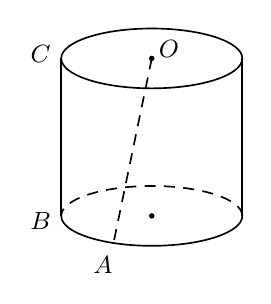
\begin{tikzpicture}[
  x=1cm, y=1cm,
  every node/.style={font=\small, inner sep=1pt},
  line/.style={line width=0.6pt},
  hidden/.style={line width=0.6pt, dash pattern=on 4pt off 3pt},
]

  % 尺寸：底面椭圆半轴、母线长
  \def\rx{1.15}
  \def\ry{0.38}
  \def\hh{2.00}

  % 下底面：前半弧实线，后半弧虚线
  \draw[line] (\rx,0) arc[start angle=0, end angle=-180, x radius=\rx, y radius=\ry];
  \draw[hidden] (\rx,0) arc[start angle=0, end angle=180, x radius=\rx, y radius=\ry];

  % 上底面整椭圆与两条母线轮廓
  \draw[line] (0,\hh) ellipse[x radius=\rx, y radius=\ry];
  \draw[line] (-\rx,0) -- (-\rx,\hh);
  \draw[line] (\rx,0) -- (\rx,\hh);

  % 母线 BC：B 在左端，C 在 B 正上方
  \draw[line] (-\rx,0) -- (-\rx,\hh);

  % 直线 OA（柱体内部，虚线）
  \draw[hidden] (0,\hh) -- (-0.486,-0.344);

  % 上、下底面圆心
  \fill (0,\hh) circle [radius=0.035];
  \fill (0,0) circle [radius=0.035];

  % 标签
  \node at (-\rx-0.26,\hh+0.06) {$C$};
  \node at (0.22,\hh+0.12) {$O$};
  \node at (-\rx-0.26,-0.06) {$B$};
  \node at (-0.62,-0.62) {$A$};

\end{tikzpicture}
\end{center}
\nopagebreak[4]
\Needspace{4\baselineskip}
\textbf{解析}
\Needspace{5\baselineskip}
建立空间直角坐标系：以下底面圆心为原点，$z$ 轴沿圆柱的轴向上，则上底面圆心 $O(0,0,l)$，下底面圆周上的点可写为 $A(r\cos\theta,r\sin\theta,0)$，$B(r\cos\varphi,r\sin\varphi,0)$。因 $BC$ 是母线，$C$ 在 $B$ 正上方，故
\nopagebreak[4]
\[\overrightarrow{OA}=(r\cos\theta,r\sin\theta,-l),\qquad \overrightarrow{BC}=(0,0,l).\]
\Needspace{5\baselineskip}
设两直线所成角为 $\alpha$，则
\nopagebreak[4]
\[\cos\alpha=\frac{\left|\overrightarrow{OA}\cdot\overrightarrow{BC}\right|}{|\overrightarrow{OA}|\cdot|\overrightarrow{BC}|}
=\frac{l}{\sqrt{r^2+l^2}}.\]
\Needspace{5\baselineskip}
已知 $\alpha=\dfrac\pi6$，故
\nopagebreak[4]
\[\frac{l}{\sqrt{r^2+l^2}}=\frac{\sqrt3}2.\]
\Needspace{5\baselineskip}
两边平方：$4l^2=3(r^2+l^2)$，即 $l^2=3r^2$，所以
\nopagebreak[4]
\[\frac lr=\sqrt3.\]

\gkanswer{答案：$\sqrt3$。取 $O(0,0,l)$，$A(r,0,0)$，则 $\overrightarrow{OA}=(r,0,-l)$，而 $\overrightarrow{BC}=(0,0,l)$，故 $\cos\dfrac\pi6=\dfrac{l}{\sqrt{r^2+l^2}}=\dfrac{\sqrt3}2$，得 $l^2=3r^2$，$\dfrac lr=\sqrt3$。}

\end{answer}
\begin{answer}
\gksolhead{11}{}

\textbf{题目}：

盒子中装有编号为 $1,2,3,4,5,6,7$ 的七个球，从中任意取出两个，则这两个球的编号之积为偶数的概率是\gkblank{}。（结果用最简分数表示）

\Needspace{4\baselineskip}
\textbf{解析}
\Needspace{5\baselineskip}
从 $7$ 个球中任取两个，共有
\nopagebreak[4]
\[\mathrm C_7^2=\frac{7\times6}{2}=21\]
\Needspace{5\baselineskip}
种等可能的取法。两球编号之积为奇数，当且仅当两球编号都是奇数。奇数编号为 $1,3,5,7$ 共 $4$ 个，取法为
\nopagebreak[4]
\[\mathrm C_4^2=6.\]
\Needspace{5\baselineskip}
故积为偶数的取法为 $21-6=15$，所求概率为
\nopagebreak[4]
\[\frac{15}{21}=\frac57.\]

\gkanswer{答案：$\dfrac57$。总取法 $\mathrm C_7^2=21$；两球编号之积为奇数须同为奇数，共 $\mathrm C_4^2=6$ 种，故积为偶数的概率为 $1-\dfrac6{21}=\dfrac57$。}

\end{answer}
\begin{answer}
\gksolhead{12}{}

\textbf{题目}：

设 $AB$ 是椭圆 $\Gamma$ 的长轴，点 $C$ 在 $\Gamma$ 上，且 $\angle CBA=\dfrac{\pi}{4}$，若 $AB=4$，$BC=\sqrt2$，则 $\Gamma$ 的两个焦点之间的距离为\gkblank{}。

\Needspace{4\baselineskip}
\textbf{解析}
\Needspace{5\baselineskip}
以长轴所在直线为 $x$ 轴、椭圆中心为原点。由 $AB=4$ 得半长轴 $a=2$，故 $A(-2,0)$，$B(2,0)$，椭圆方程为
\nopagebreak[4]
\[\frac{x^2}4+\frac{y^2}{b^2}=1\quad(0<b<2).\]
\Needspace{5\baselineskip}
射线 $BA$ 沿 $x$ 轴负方向，$\angle CBA=\dfrac\pi4$ 表示 $BC$ 与负 $x$ 轴成 $\dfrac\pi4$ 角，结合 $BC=\sqrt2$ 得
\nopagebreak[4]
\[C=\left(2-\sqrt2\cos\frac\pi4,\ \pm\sqrt2\sin\frac\pi4\right)=(1,\pm1).\]
\Needspace{5\baselineskip}
把 $C(1,1)$ 代入椭圆方程：
\nopagebreak[4]
\[\frac14+\frac1{b^2}=1,\]
\Needspace{5\baselineskip}
解得 $b^2=\dfrac43$。于是
\nopagebreak[4]
\[c^2=a^2-b^2=4-\frac43=\frac83,\qquad c=\frac{2\sqrt6}3,\]
\Needspace{5\baselineskip}
两焦点之间的距离为
\nopagebreak[4]
\[2c=\frac{4\sqrt6}3.\]
数值复核：$\dfrac{4\sqrt6}3\approx3.266<4=2a$，符合椭圆中焦距小于长轴长。

\gkanswer{答案：$\dfrac{4\sqrt6}3$。设椭圆为 $\dfrac{x^2}4+\dfrac{y^2}{b^2}=1$，$B(2,0)$，则 $\angle CBA=\dfrac\pi4$ 且 $BC=\sqrt2$ 给出 $C(1,\pm1)$；代入得 $\dfrac14+\dfrac1{b^2}=1$，$b^2=\dfrac43$，于是 $c^2=4-\dfrac43=\dfrac83$，两焦点距离 $2c=\dfrac{4\sqrt6}3$。}

\end{answer}
\begin{answer}
\gksolhead{13}{}

\textbf{题目}：

设常数 $a>0$。若 $9x+\dfrac{a^2}{x}\geqslant a+1$ 对一切正实数 $x$ 成立，则 $a$ 的取值范围为\gkblank{}。

\Needspace{4\baselineskip}
\textbf{解析}
\Needspace{5\baselineskip}
对 $x>0$，由均值不等式
\nopagebreak[4]
\[9x+\frac{a^2}x\geqslant2\sqrt{9x\cdot\frac{a^2}x}=2\sqrt{9a^2}=6a,\]
\Needspace{5\baselineskip}
等号当且仅当 $9x=\dfrac{a^2}x$，即 $x=\dfrac a3$ 时取得（$a>0$，该点为正实数）。因此
\nopagebreak[4]
\[\min_{x>0}\left(9x+\frac{a^2}x\right)=6a.\]
\Needspace{5\baselineskip}
题设要求该最小值不小于 $a+1$：
\nopagebreak[4]
\[6a\geqslant a+1\iff a\geqslant\frac15.\]
故 $a$ 的取值范围为 $\left[\dfrac15,+\infty\right)$。

\gkanswer{答案：$\left[\dfrac15,+\infty\right)$。由均值不等式 $9x+\dfrac{a^2}x\geqslant2\sqrt{9a^2}=6a$（等号在 $x=\dfrac a3$ 取得），故只需 $6a\geqslant a+1$，即 $a\geqslant\dfrac15$。}

\end{answer}
\begin{answer}
\gksolhead{14}{}

\textbf{题目}：

已知正方形 $ABCD$ 的边长为 $1$。记以 $A$ 为起点，其余顶点为终点的向量分别为 $\overrightarrow{a_1}$、$\overrightarrow{a_2}$、$\overrightarrow{a_3}$；以 $C$ 为起点，其余顶点为终点的向量分别为 $\overrightarrow{c_1}$、$\overrightarrow{c_2}$、$\overrightarrow{c_3}$。若 $i,j,k,l\in\{1,2,3\}$ 且 $i\neq j$，$k\neq l$，则 $(\overrightarrow{a_i}+\overrightarrow{a_j})\cdot(\overrightarrow{c_k}+\overrightarrow{c_l})$ 的最小值是\gkblank{}。

\Needspace{4\baselineskip}
\textbf{解析}
\Needspace{5\baselineskip}
取坐标系 $A(0,0)$，$B(1,0)$，$C(1,1)$，$D(0,1)$。以 $A$ 为起点的三个向量为
\nopagebreak[4]
\[\overrightarrow{AB}=(1,0),\quad\overrightarrow{AC}=(1,1),\quad\overrightarrow{AD}=(0,1);\]
\Needspace{5\baselineskip}
以 $C$ 为起点的三个向量为
\nopagebreak[4]
\[\overrightarrow{CA}=(-1,-1),\quad\overrightarrow{CB}=(0,-1),\quad\overrightarrow{CD}=(-1,0).\]
\Needspace{5\baselineskip}
两个不同的 $\overrightarrow{a}$ 之和只有三种：
\nopagebreak[4]
\[(1,0)+(1,1)=(2,1),\quad(1,0)+(0,1)=(1,1),\quad(1,1)+(0,1)=(1,2);\]
\Needspace{5\baselineskip}
两个不同的 $\overrightarrow{c}$ 之和也只有三种：
\nopagebreak[4]
\[\begin{aligned}
(-1,-1)+(0,-1)&=(-1,-2),\\
(-1,-1)+(-1,0)&=(-2,-1),\\
(0,-1)+(-1,0)&=(-1,-1).
\end{aligned}\]
逐一作内积：

\begin{center}
\begin{tabular}{llll}
\toprule
和向量 & $(-1,-2)$ & $(-2,-1)$ & $(-1,-1)$ \\
\midrule
$(2,1)$ & $-4$ & $-5$ & $-3$ \\
$(1,1)$ & $-3$ & $-3$ & $-2$ \\
$(1,2)$ & $-5$ & $-4$ & $-3$ \\
\bottomrule
\end{tabular}
\end{center}

最小值为 $-5$，在 $(2,1)$ 与 $(-2,-1)$ 或 $(1,2)$ 与 $(-1,-2)$ 时取得。注意题设只要求 $i\neq j$、$k\neq l$，并不要求四者互不相同，故上表全部组合都允许。

\gkanswer{答案：$-5$。}

\end{answer}
\begin{answer}
\gksolhead{15}{}

\textbf{题目}：

函数 $f(x)=x^2-1$（$x\geqslant 1$）的反函数为 $f^{-1}(x)$，则 $f^{-1}(2)$ 的值是\mbox{（　　）}

（A）$\sqrt3$；（B）$-\sqrt3$；（C）$1+\sqrt2$；（D）$1-\sqrt2$。

\Needspace{4\baselineskip}
\textbf{解析}
\Needspace{5\baselineskip}
由 $y=x^2-1$ 且 $x\geqslant1$ 得 $x^2=y+1$，因 $x>0$ 取正根：
\nopagebreak[4]
\[x=\sqrt{y+1}.\]
\Needspace{5\baselineskip}
故反函数为 $f^{-1}(x)=\sqrt{x+1}$（定义域 $x\geqslant-1$），于是
\nopagebreak[4]
\[f^{-1}(2)=\sqrt{2+1}=\sqrt3.\]
验证：$f(\sqrt3)=3-1=2$。

\gkanswer{答案：A。由 $y=x^2-1$（$x\geqslant1$）解得 $x=\sqrt{y+1}$，即 $f^{-1}(x)=\sqrt{x+1}$，故 $f^{-1}(2)=\sqrt3$。}

\end{answer}
\begin{answer}
\gksolhead{16}{}

\textbf{题目}：

设常数 $a\in\mathbf R$，集合 $A=\{x\mid (x-1)(x-a)\geqslant 0\}$，$B=\{x\mid x\geqslant a-1\}$。若 $A\cup B=\mathbf R$，则 $a$ 的取值范围为\mbox{（　　）}

（A）$(-\infty,2)$；（B）$(-\infty,2]$；（C）$(2,+\infty)$；（D）$[2,+\infty)$。

\Needspace{4\baselineskip}
\textbf{解析}
按 $a$ 与 $1$ 的大小分两类。

\Needspace{5\baselineskip}
若 $a\geqslant1$，则 $(x-1)(x-a)\geqslant0$ 的解为
\nopagebreak[4]
\[A=(-\infty,1]\cup[a,+\infty),\]
\Needspace{5\baselineskip}
又 $B=[a-1,+\infty)$。要使 $A\cup B=\mathbf R$，必须且只需区间 $(1,a)$ 被 $B$ 覆盖，即
\nopagebreak[4]
\[a-1\leqslant1\iff a\leqslant2.\]
此时 $1\leqslant a\leqslant2$ 均满足。

\Needspace{5\baselineskip}
若 $a<1$，则
\nopagebreak[4]
\[A=(-\infty,a]\cup[1,+\infty),\]
而 $B=[a-1,+\infty)$ 的左端点 $a-1<a$，故 $(a,1)\subset B$，从而 $A\cup B=\mathbf R$ 恒成立。

综上 $a\leqslant2$，取值范围为 $(-\infty,2]$。检验端点：$a=2$ 时 $A=(-\infty,1]\cup[2,+\infty)$，$B=[1,+\infty)$，并集为 $\mathbf R$；$a=3$ 时并集遗漏 $(1,2)$。

\gkanswer{答案：B。若 $a\geqslant1$，则 $A=(-\infty,1]\cup[a,+\infty)$，$B=[a-1,+\infty)$，$A\cup B=\mathbf R$ 需 $a-1\leqslant1$，即 $1\leqslant a\leqslant2$；若 $a<1$，则 $A=(-\infty,a]\cup[1,+\infty)$，而 $(a,1)\subset[a-1,+\infty)=B$，恒有 $A\cup B=\mathbf R$。故 $a\leqslant2$。}

\end{answer}
\begin{answer}
\gksolhead{17}{}

\textbf{题目}：

钱大姐常说“便宜没好货”，她这句话的意思是：“不便宜”是“好货”的\mbox{（　　）}

（A）充分条件；（B）必要条件；（C）充分必要条件；（D）既非充分也非必要条件。

\Needspace{4\baselineskip}
\textbf{解析}
\Needspace{5\baselineskip}
“便宜没好货”的含义是：若一件货便宜，则它不是好货，即
\nopagebreak[4]
\[\text{\text{便宜}}\Rightarrow\text{\text{不是好货}}.\]
\Needspace{5\baselineskip}
其逆否命题为
\nopagebreak[4]
\[\text{\text{好货}}\Rightarrow\text{\text{不便宜}}.\]
所以“好货”能推出“不便宜”，即“不便宜”是“好货”的必要条件；但“不便宜”未必是“好货”（贵而劣质者存在），故不是充分条件。选 B。

\gkanswer{答案：B。“便宜没好货”即“便宜”推出“不是好货”，其逆否命题为“好货”推出“不便宜”，故“不便宜”是“好货”的必要条件。}

\end{answer}
\begin{answer}
\gksolhead{18}{}

\textbf{题目}：

记椭圆 $\dfrac{x^2}{4}+\dfrac{ny^2}{4n+1}=1$ 围成的区域（含边界）为 $\Omega_n$（$n=1,2,\cdots$），当点 $(x,y)$ 分别在 $\Omega_1$，$\Omega_2$，$\cdots$ 上时，$x+y$ 的最大值分别是 $M_1$，$M_2$，$\cdots$，则 $\lim\limits_{n\to\infty}M_n=$\mbox{（　　）}

（A）$0$；（B）$\dfrac14$；（C）$2$；（D）$2\sqrt2$。

\Needspace{4\baselineskip}
\textbf{解析}
\Needspace{5\baselineskip}
$\Omega_n$ 是椭圆 $\dfrac{x^2}4+\dfrac{ny^2}{4n+1}=1$ 及其内部，半轴为
\nopagebreak[4]
\[a=2,\qquad b_n=\sqrt{\frac{4n+1}{n}}.\]
\Needspace{5\baselineskip}
令 $x=2\cos\theta$，$y=b_n\sin\theta$，则
\nopagebreak[4]
\[x+y=2\cos\theta+b_n\sin\theta\leqslant\sqrt{2^2+b_n^2},\]
\Needspace{5\baselineskip}
等号在 $(\cos\theta,\sin\theta)$ 与 $(2,b_n)$ 同向时取得，故
\nopagebreak[4]
\[M_n=\sqrt{4+b_n^2}=\sqrt{4+\frac{4n+1}{n}}=\sqrt{8+\frac1n}.\]
\Needspace{5\baselineskip}
于是
\nopagebreak[4]
\[\lim_{n\to\infty}M_n=\sqrt8=2\sqrt2.\]

\gkanswer{答案：D。$\Omega_n$ 的半轴为 $2$ 与 $\sqrt{\dfrac{4n+1}{n}}$，故 $M_n=\sqrt{4+\dfrac{4n+1}{n}}=\sqrt{8+\dfrac1n}\to2\sqrt2$。}

\end{answer}
\begin{answer}
\gksolhead{19}{}

\textbf{题目}：

如图，正三棱锥 $O-ABC$ 底面边长为 $2$，高为 $1$，求该三棱锥的体积及表面积。
\nopagebreak[4]
\begin{center}% ============================================================
% f2013_shanghai_arts_q19_pyramid.tex
% 2013 上海卷（文科）第 19 题 正三棱锥 O-ABC（TikZ 矢量重绘）
% 几何：底面为边长为 2 的正三角形 ABC，顶点 O 在底面上的射影为底面中心，
%       高为 1。AB 为被遮挡的底面棱，画虚线；其余各棱实线。
% ============================================================
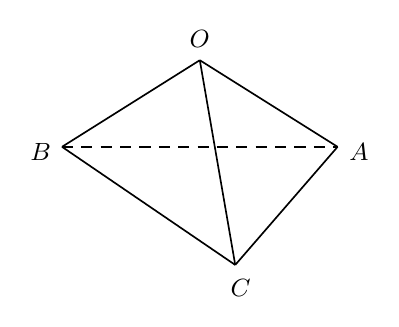
\begin{tikzpicture}[
  x=1cm, y=1cm,
  every node/.style={font=\small, inner sep=1pt},
  line/.style={line width=0.6pt},
  hidden/.style={line width=0.6pt, dash pattern=on 4pt off 3pt},
]

  \coordinate (O) at (0,3.05);
  \coordinate (B) at (-1.75,1.95);
  \coordinate (A) at (1.75,1.95);
  \coordinate (C) at (0.45,0.45);

  % 侧棱
  \draw[line] (O) -- (A);
  \draw[line] (O) -- (B);
  \draw[line] (O) -- (C);

  % 底面棱：AB 被遮挡
  \draw[hidden] (B) -- (A);
  \draw[line] (B) -- (C);
  \draw[line] (C) -- (A);

  % 标签
  \node at (0,3.32) {$O$};
  \node at (-2.02,1.88) {$B$};
  \node at (2.02,1.88) {$A$};
  \node at (0.52,0.16) {$C$};

\end{tikzpicture}
\end{center}
\nopagebreak[4]
\Needspace{4\baselineskip}
\textbf{解析}
\Needspace{5\baselineskip}
设底面中心为 $H$，则 $OH\perp$ 底面，$OH=1$。底面是边长为 $2$ 的正三角形，面积
\nopagebreak[4]
\[S_{\triangle ABC}=\frac{\sqrt3}4\cdot2^2=\sqrt3.\]
\Needspace{5\baselineskip}
体积
\nopagebreak[4]
\[V=\frac13 S_{\triangle ABC}\cdot OH=\frac13\cdot\sqrt3\cdot1=\frac{\sqrt3}3.\]

\Needspace{5\baselineskip}
再求表面积。$H$ 是正三角形的中心，它到任一边的距离等于正三角形的内切圆半径
\nopagebreak[4]
\[r_{\text{\text{内}}}=\frac{\sqrt3}6\times2=\frac{\sqrt3}3.\]
\Needspace{5\baselineskip}
取 $BC$ 的中点 $M$，则 $HM\perp BC$，$HM=\dfrac{\sqrt3}3$，且 $OH\perp HM$，故斜高
\nopagebreak[4]
\[OM=\sqrt{OH^2+HM^2}=\sqrt{1+\frac13}=\frac{2}{\sqrt3}=\frac{2\sqrt3}3.\]
\Needspace{5\baselineskip}
于是
\nopagebreak[4]
\[S_{\triangle OBC}=\frac12\cdot BC\cdot OM=\frac12\cdot2\cdot\frac{2\sqrt3}3=\frac{2\sqrt3}3,\]
\Needspace{5\baselineskip}
三个侧面全等，侧面积为 $3\cdot\dfrac{2\sqrt3}3=2\sqrt3$。故表面积
\nopagebreak[4]
\[S=S_{\triangle ABC}+3S_{\triangle OBC}=\sqrt3+2\sqrt3=3\sqrt3.\]

\gkanswer{答案：$V=\dfrac{\sqrt3}3$，$S=3\sqrt3$。}

\end{answer}
\begin{answer}
\gksolhead{20}{}

\textbf{题目}：

甲厂以 $x$ 千克/小时的速度运输生产某种产品（生产条件要求 $1\leqslant x\leqslant 10$），每一小时可获得利润是 $100\left(5x+1-\dfrac3x\right)$ 元。

（1） 求证：生产 $a$ 千克该产品所获得的利润为 $100a\left(5+\dfrac1x-\dfrac{3}{x^2}\right)$ 元；

（2） 要使生产 $900$ 千克该产品获得的利润最大，问：甲厂应该选取何种生产速度？并求最大利润。

\Needspace{4\baselineskip}
\textbf{解析}
\Needspace{5\baselineskip}
\textbf{（1）} 生产 $a$ 千克产品所需时间为 $\dfrac ax$ 小时（$x>0$），每小时的利润为 $100\left(5x+1-\dfrac3x\right)$ 元，故总利润为
\nopagebreak[4]
\[\frac ax\cdot100\left(5x+1-\frac3x\right)=100a\left(5+\frac1x-\frac{3}{x^2}\right)\ \text{\text{元}}.\]
这就是要证的表达式。

\Needspace{5\baselineskip}
\textbf{（2）} 取 $a=900$，总利润为
\nopagebreak[4]
\[P(x)=90000\left(5+\frac1x-\frac{3}{x^2}\right),\qquad 1\leqslant x\leqslant10.\]
\Needspace{5\baselineskip}
令 $u=\dfrac1x$，则 $x\in[1,10]$ 对应 $u\in\left[\dfrac1{10},1\right]$，且
\nopagebreak[4]
\[P=90000\left(5+u-3u^2\right).\]
\Needspace{5\baselineskip}
二次函数 $5+u-3u^2$ 的图象开口向下，对称轴为
\nopagebreak[4]
\[u=-\frac{1}{2\times(-3)}=\frac16,\]
\Needspace{5\baselineskip}
且 $\dfrac16\in\left[\dfrac1{10},1\right]$，故最大值在 $u=\dfrac16$ 处取得，即 $x=6$。此时
\nopagebreak[4]
\[\begin{aligned}
5+\frac16-3\cdot\frac1{36}
&=5+\frac16-\frac1{12}\\
&=5+\frac1{12}=\frac{61}{12},
\end{aligned}\]
\nopagebreak[4]
\[P_{\max}=90000\times\frac{61}{12}=7500\times61=457500.\]
端点比较：$x=1$（$u=1$）时 $P=90000\times3=270000$；$x=10$（$u=0.1$）时 $P=90000\times5.07=456300$，均小于 $457500$。故甲厂应选取 $6$ 千克/小时的生产速度，最大利润为 $457500$ 元。

\gkanswer{答案（1）：证明见解析。}

\gkanswer{答案（2）：$x=6$ 千克/小时，最大利润 $457500$ 元。}

\end{answer}
\begin{answer}
\gksolhead{21}{}

\textbf{题目}：

已知函数 $f(x)=2\sin\omega x$，其中常数 $\omega>0$。

（1） 令 $\omega=1$，判断函数 $F(x)=f(x)+f\left(x+\dfrac{\pi}{2}\right)$ 的奇偶性并说明理由；

（2） 令 $\omega=2$，将函数 $y=f(x)$ 的图象向左平移 $\dfrac{\pi}{6}$ 个单位，再向上平移 $1$ 个单位，得到函数 $y=g(x)$ 的图象。对任意的 $a\in\mathbf R$，求 $y=g(x)$ 在区间 $[a,a+10\pi]$ 上零点个数的所有可能值。

\Needspace{4\baselineskip}
\textbf{解析}
\Needspace{5\baselineskip}
\textbf{（1）} 当 $\omega=1$ 时 $f(x)=2\sin x$，于是
\nopagebreak[4]
\[F(x)=2\sin x+2\sin\left(x+\frac\pi2\right)=2\sin x+2\cos x=2\sqrt2\sin\left(x+\frac\pi4\right).\]
\Needspace{5\baselineskip}
定义域为 $\mathbf R$，关于原点对称。计算
\nopagebreak[4]
\[F(0)=2\sqrt2\sin\frac\pi4=2\neq0,\]
\Needspace{5\baselineskip}
故 $F$ 不是奇函数（奇函数在 $0$ 处必须取 $0$）。又
\nopagebreak[4]
\[F\left(\frac\pi2\right)=2\sqrt2\sin\frac{3\pi}4=2,\qquad
F\left(-\frac\pi2\right)=2\sqrt2\sin\left(-\frac\pi4\right)=-2,\]
两者不相等，故 $F$ 不是偶函数。所以 $F(x)$ 既不是奇函数也不是偶函数。

\Needspace{5\baselineskip}
\textbf{（2）} 当 $\omega=2$ 时 $f(x)=2\sin2x$。图象向左平移 $\dfrac\pi6$ 个单位得 $y=2\sin2\left(x+\dfrac\pi6\right)=2\sin\left(2x+\dfrac\pi3\right)$，再向上平移 $1$ 个单位得
\nopagebreak[4]
\[g(x)=2\sin\left(2x+\frac\pi3\right)+1.\]
\Needspace{5\baselineskip}
零点满足
\nopagebreak[4]
\[\sin\left(2x+\frac\pi3\right)=-\frac12,\]
\Needspace{5\baselineskip}
故
\nopagebreak[4]
\[2x+\frac\pi3=-\frac\pi6+2k\pi\quad\text{\text{或}}\quad 2x+\frac\pi3=\frac{7\pi}6+2k\pi,\]
\Needspace{5\baselineskip}
即
\nopagebreak[4]
\[x=-\frac\pi4+k\pi\quad\text{\text{或}}\quad x=\frac{5\pi}{12}+k\pi,\qquad k\in\mathbf Z.\]
记零点集合为 $Z$。$g$ 的周期为 $\pi$，且 $Z+\pi=Z$，故把区间 $[a,a+10\pi]$ 整体平移整数个周期不改变零点个数，可设 $a\in[0,\pi)$。

$Z$ 由两个公差为 $\pi$ 的等差数列组成。任意长度为 $10\pi$（恰为 $10$ 个周期）的半开区间 $[a,a+10\pi)$ 中，每个数列恰有 $10$ 项，共 $20$ 个零点。再考察右端点 $a+10\pi$：由于 $Z+\pi=Z$，$a+10\pi\in Z$ 当且仅当 $a\in Z$。因此

\begin{itemize}
\item 当 $a\notin Z$ 时，$[a,a+10\pi]$ 内零点个数为 $20$；
\item 当 $a\in Z$ 时，$a$ 与 $a+10\pi$ 都是零点，个数为 $21$。
\end{itemize}

相邻零点的间距交替为 $\dfrac{2\pi}3$ 与 $\dfrac\pi3$（例如 $-\dfrac\pi4$ 与 $\dfrac{5\pi}{12}$ 相距 $\dfrac{2\pi}3$，$\dfrac{5\pi}{12}$ 与 $\dfrac{3\pi}4$ 相距 $\dfrac\pi3$），故两种情形都能取到。所以零点个数的所有可能值为 $20$ 或 $21$。

\gkanswer{答案（1）：既不是奇函数也不是偶函数。}

\gkanswer{答案（2）：$20$ 或 $21$。}

\end{answer}
\begin{answer}
\gksolhead{22}{}

\textbf{题目}：

已知函数 $f(x)=2-|x|$，无穷数列 $\{a_n\}$ 满足 $a_{n+1}=f(a_n)$，$n\in\mathbf N^*$。

（1） 若 $a_1=0$，求 $a_2$，$a_3$，$a_4$；

（2） 若 $a_1>0$，且 $a_1$，$a_2$，$a_3$ 成等比数列，求 $a_1$ 的值；

（3） 是否存在 $a_1$，使得 $a_1$，$a_2$，$a_3$，$\cdots$，$a_n$，$\cdots$ 成等差数列？若存在，求出所有这样的 $a_1$；若不存在，说明理由。

\Needspace{4\baselineskip}
\textbf{解析}
\Needspace{5\baselineskip}
\textbf{（1）} 依次计算：
\nopagebreak[4]
\[a_2=2-|a_1|=2-0=2,\qquad a_3=2-|2|=0,\qquad a_4=2-|0|=2.\]

\textbf{（2）} 由 $a_1>0$，分两种情形。

\Needspace{5\baselineskip}
若 $0<a_1\leqslant2$，则 $a_2=2-|a_1|=2-a_1\geqslant0$，从而 $a_3=2-|a_2|=2-a_2=a_1$。等比条件 $a_2^2=a_1a_3$ 化为
\nopagebreak[4]
\[(2-a_1)^2=a_1^2\iff4-4a_1+a_1^2=a_1^2\iff a_1=1.\]
此时 $a_1=a_2=a_3=1$，公比为 $1$，符合要求。

\Needspace{5\baselineskip}
若 $a_1>2$，则 $a_2=2-a_1<0$，$|a_2|=a_1-2$，故
\nopagebreak[4]
\[a_3=2-|a_2|=2-(a_1-2)=4-a_1.\]
\Needspace{5\baselineskip}
等比条件为
\nopagebreak[4]
\[(2-a_1)^2=a_1(4-a_1),\]
\Needspace{5\baselineskip}
展开得 $4-4a_1+a_1^2=4a_1-a_1^2$，即
\nopagebreak[4]
\[a_1^2-4a_1+2=0,\]
\Needspace{5\baselineskip}
解得 $a_1=2\pm\sqrt2$。因 $a_1>2$，取 $a_1=2+\sqrt2$。此时
\nopagebreak[4]
\[a_1=2+\sqrt2,\quad a_2=-\sqrt2,\quad a_3=2-\sqrt2,\]
公比 $q=\dfrac{a_2}{a_1}=1-\sqrt2$，且 $\dfrac{a_3}{a_2}=1-\sqrt2$，符合要求。

综上 $a_1=1$ 或 $a_1=2+\sqrt2$。

\textbf{（3）} 存在，且只有 $a_1=1$。证明如下。

对任意 $x$，$f(x)=2-|x|\leqslant2$，故 $n\geqslant2$ 时 $a_n\leqslant2$。设 $\{a_n\}$ 是公差为 $d$ 的等差数列。

若 $d>0$，则 $a_n=a_1+(n-1)d\to+\infty$，与 $a_n\leqslant2$（$n\geqslant2$）矛盾，故 $d\leqslant0$。

\Needspace{5\baselineskip}
若 $d<0$，则 $a_n\to-\infty$，存在 $N$ 使 $n\geqslant N$ 时 $a_n<0$。此时 $|a_n|=-a_n$，于是
\nopagebreak[4]
\[a_{n+1}=2-|a_n|=2+a_n\Longrightarrow a_{n+1}-a_n=2,\]
与公差 $d<0$ 矛盾。故 $d=0$。

\Needspace{5\baselineskip}
于是 $a_n$ 恒等于某个常数 $c$，且
\nopagebreak[4]
\[c=2-|c|.\]
若 $c\geqslant0$，则 $c=2-c$，$c=1$；若 $c<0$，则 $c=2+c$，即 $0=2$，无解。故 $c=1$，从而 $a_1=1$。

反之，当 $a_1=1$ 时 $a_2=2-|1|=1$，归纳得 $a_n=1$ 对一切 $n$ 成立，这是公差为 $0$ 的等差数列。故存在唯一的 $a_1=1$。

\gkanswer{答案（1）：$a_2=2$，$a_3=0$，$a_4=2$。}

\gkanswer{答案（2）：$a_1=1$ 或 $a_1=2+\sqrt2$。}

\gkanswer{答案（3）：存在，$a_1=1$。}

\end{answer}
\begin{answer}
\gksolhead{23}{}

\textbf{题目}：

如图，已知双曲线 $C_1:\dfrac{x^2}{2}-y^2=1$，曲线 $C_2:|y|=|x|+1$。$P$ 是平面内一点，若存在过点 $P$ 的直线与 $C_1$、$C_2$ 都有公共点，则称 $P$ 为“$C_1-C_2$ 型点”。
\nopagebreak[4]
\begin{center}% ============================================================
% f2013_shanghai_arts_q23_hyperbola.tex
% 2013 上海卷（文科）第 23 题 双曲线 C1 与折线 C2（TikZ 矢量重绘）
% 曲线：C1: x^2/2 - y^2 = 1（两支，顶点在 (±sqrt2, 0)）；
%       C2: |y| = |x| + 1（两条折线，顶点分别在 (0,1)、(0,-1)，四臂斜率 ±1）。
% 坐标轴等比例，便于看出 C1 渐近线 y = ±x/sqrt2 与 C2 四臂的方向差别。
% ============================================================
\begin{tikzpicture}[
  x=1.1cm, y=1.1cm,
  every node/.style={font=\small, inner sep=1pt},
  line/.style={line width=0.6pt},
  axis/.style={line width=0.5pt, -{Stealth[length=2.2mm,width=1.6mm]}},
]

  % 坐标轴
  \draw[axis] (-3.25,0) -- (3.45,0);
  \draw[axis] (0,-2.85) -- (0,3.05);

  % C1 的左右两支：x = ±sqrt(2(1+t^2)), y = t
  \draw[line, domain=-2.03:2.03, samples=120, smooth, variable=\t]
    plot ({sqrt(2*(1+\t*\t))}, {\t});
  \draw[line, domain=-2.03:2.03, samples=120, smooth, variable=\t]
    plot ({-sqrt(2*(1+\t*\t))}, {\t});

  % C2 的两条折线：|y| = |x| + 1
  \draw[line] (-1.92,2.92) -- (0,1) -- (1.92,2.92);
  \draw[line] (-1.92,-2.92) -- (0,-1) -- (1.92,-2.92);

  % 原点与轴标签
  \node at (-0.34,-0.38) {$O$};
  \node at (3.62,-0.24) {$x$};
  \node at (-0.26,3.22) {$y$};

\end{tikzpicture}
\end{center}
\nopagebreak[4]
（1） 在正确证明 $C_1$ 的左焦点是“$C_1-C_2$ 型点”时，要使用一条过该焦点的直线，试写出一条这样的直线的方程（不要求验证）；

（2） 设直线 $y=kx$ 与 $C_2$ 有公共点，求证 $|k|>1$，进而证明原点不是“$C_1-C_2$ 型点”；

（3） 求证：圆 $x^2+y^2=\dfrac12$ 内的点都不是“$C_1-C_2$ 型点”。

\Needspace{4\baselineskip}
\textbf{解析}
\Needspace{5\baselineskip}
\textbf{（1）} $C_1$ 中 $a^2=2$，$b^2=1$，故 $c^2=a^2+b^2=3$，左焦点为 $F(-\sqrt3,0)$。取过 $F$ 的直线
\nopagebreak[4]
\[x=-\sqrt3.\]
它与 $C_1$ 的交点满足 $\dfrac32-y^2=1$，即 $y=\pm\dfrac{\sqrt2}2$，有公共点；它与 $C_2$ 的交点满足 $|y|=\sqrt3+1$，即 $y=\pm(1+\sqrt3)$，也有公共点。故 $x=-\sqrt3$ 即为所求（题设不要求验证）。

\Needspace{5\baselineskip}
\textbf{（2）} 设 $y=kx$ 与 $C_2$ 有公共点 $(x,y)$。若 $x=0$，则 $|y|=1$，但 $y=k\cdot0=0$，矛盾，故 $x\neq0$。代入 $|y|=|x|+1$ 得
\nopagebreak[4]
\[|k|\,|x|=|x|+1\Longrightarrow |x|\left(|k|-1\right)=1.\]
\Needspace{5\baselineskip}
因 $|x|>0$，必须 $|k|-1>0$，即
\nopagebreak[4]
\[|k|>1.\]

再证原点不是“$C_1-C_2$ 型点”。过原点的直线分两类。

\Needspace{5\baselineskip}
若直线为 $y=kx$ 且与 $C_2$ 有公共点，由上一段得 $|k|>1$。代入 $C_1$：
\nopagebreak[4]
\[\frac{x^2}2-k^2x^2=1\Longrightarrow x^2\left(\frac12-k^2\right)=1.\]
因 $k^2>1>\dfrac12$，左端 $\leqslant0$，方程无实根，故该直线与 $C_1$ 无公共点。

若直线为 $y$ 轴 $x=0$，代入 $C_1$ 得 $-y^2=1$，无实根，与 $C_1$ 无公共点。

所以不存在过原点且与 $C_1$、$C_2$ 都有公共点的直线，原点不是“$C_1-C_2$ 型点”。

\textbf{（3）} 设 $P(x_0,y_0)$ 满足 $x_0^2+y_0^2<\dfrac12$，$l$ 是过 $P$ 的直线。

\Needspace{5\baselineskip}
若 $l$ 的斜率不存在，则 $l:x=x_0$。因
\nopagebreak[4]
\[|x_0|\leqslant\sqrt{x_0^2+y_0^2}<\frac1{\sqrt2}<\sqrt2,\]
故 $\dfrac{x_0^2}2<1$，而 $C_1$ 上的点满足 $\dfrac{x^2}2=1+y^2\geqslant1$，所以 $l$ 与 $C_1$ 无公共点。

\Needspace{5\baselineskip}
以下设 $l:y=kx+m$。原点 $O$ 到 $l$ 的距离为 $\dfrac{|m|}{\sqrt{1+k^2}}$，而 $l$ 过 $P$，故该距离不超过 $|OP|$：
\nopagebreak[4]
\[\frac{|m|}{\sqrt{1+k^2}}\leqslant|OP|<\frac1{\sqrt2}\Longrightarrow m^2<\frac{1+k^2}2.\]

\Needspace{5\baselineskip}
若 $|k|\leqslant1$，则 $m^2<\dfrac{1+k^2}2\leqslant1$，即 $|m|<1$。对 $l$ 上任意点 $(x,kx+m)$，
\nopagebreak[4]
\[|y|=|kx+m|\leqslant|k|\,|x|+|m|<|x|+1,\]
故 $l$ 上不存在满足 $|y|=|x|+1$ 的点，$l$ 与 $C_2$ 无公共点。

\Needspace{5\baselineskip}
若 $|k|>1$，把 $y=kx+m$ 代入 $C_1$：
\nopagebreak[4]
\[\frac{x^2}2-(kx+m)^2=1,\]
\Needspace{5\baselineskip}
整理得
\nopagebreak[4]
\[\left(1-2k^2\right)x^2-4kmx-2\left(m^2+1\right)=0.\]
\Needspace{5\baselineskip}
其判别式为
\nopagebreak[4]
\[\Delta=16k^2m^2+8\left(1-2k^2\right)\left(m^2+1\right)=8\left(m^2+1-2k^2\right).\]
\Needspace{5\baselineskip}
由 $m^2<\dfrac{1+k^2}2$ 得
\nopagebreak[4]
\[\Delta<8\left(\frac{1+k^2}2+1-2k^2\right)=4\left(3-3k^2\right)<0,\]
故方程无实根，$l$ 与 $C_1$ 无公共点。

综上，过圆 $x^2+y^2=\dfrac12$ 内任一点的直线不可能同时与 $C_1$、$C_2$ 有公共点，即圆内的点都不是“$C_1-C_2$ 型点”。

\gkanswer{答案（1）：$x=-\sqrt3$（答案不唯一）。}

\gkanswer{答案（2）：证明见解析。}

\gkanswer{答案（3）：证明见解析。}

\end{answer}